\documentclass[12pt]{article}

% Language setting
\usepackage[utf8]{inputenc}
\usepackage[bulgarian]{babel}

% --------------------- Packages  --------------------
% Use biblatex
\usepackage{biblatex}
\addbibresource{bibliography.bib}
% Table thickness
\usepackage{ctable}
% Equations: SI units
\usepackage{siunitx}
% Approximately equal
\usepackage{amssymb}
% degrees symbol
\usepackage{gensymb}
% warning box
\usepackage{pifont,mdframed}
% Multiline math
\usepackage{amsmath}

\newenvironment{warning}
  {\par\begin{mdframed}[linewidth=2pt, linecolor=white]%
    \begin{list}{}{\leftmargin=1cm
                   \labelwidth=\leftmargin}\item[\Large\ding{43}]}
  {\end{list}\end{mdframed}\par}

% --------------------- Title  --------------------
\addbibresource{bibliography.bib}

\begin{document}

% Anfang der Titelseite________________________________________________________________________________
\begin{titlepage}
	\flushleft
	{\scshape\Large Протокол IX \hspace{2cm} Молекулна физика\par}
	\vspace{4cm}
	{\huge\bfseries Измерване на дължината на средния свободен пробег на молекулите на въздух\par}
	\vspace{1cm}
	{\LARGE\bfseries Лабораторно упражнение №3.2\par}
	\vspace{5cm}
    {\LARGE\bfseries Виолета Кабаджова, \par}
    {\large\bfseries ККТФ, фак. номер: 3PH0600026\par}
	\vspace{1cm}
	
	{\large Физически Факултет, 
	
	Софийски Университет "Св. Климент Охридски"
	
	28 май 2023 г.\par}
	
\end{titlepage}

\section{Теоритична част}\label{sec:theoretical-part}
При движението на един реален флуид възникват сили на вътрешно триене, които се описват чрез ур. \ref{eq:newton}, където $\eta$ - коефициент на вътрешно триене, $\left| \frac{\Delta v}{\Delta y}\right|$ - изменението на големината на скоростта, $S$ - площта на триещите се слоеве. 

\begin{equation}\label{eq:newton}
    F = \eta \left| \frac{\Delta v}{\Delta y}\right| S
\end{equation}
Изследваме флуид в тръба, и тъй като той се движи под действие на разликата в налягания в двата края на тръбата, то потокът, който преминава през тръба, може да се опише посредством закона на Поазьой \ref{eq:stream}.

Използвайки формулата за потока флуид Q, преминаващ през тръбата, (закон на Поазьой \ref{eq:stream}), обема на изтеклия през тръбата флуид за време $t$ (формила \ref{eq:V}), както и изразяването на $\Delta p$ под формата \ref{eq:delta-p}, получаваме работната ни формула \ref{eq:work-formula} за коефициента на вътрешно триене $\eta$, която зависи от променливите $V$, $t$, $\Delta h$, които можем да измерим пряко при протичането на количество флуид през тръба.

\begin{equation}\label{eq:delta-p}
    \Delta p = p_1 - p_2 = \rho g h_1 - \rho g h_2 = \rho g \Delta h
\end{equation}

\begin{equation}\label{eq:stream}
    Q = \frac{\Delta p}{8 \eta l} \pi r^4
\end{equation}

\begin{equation}\label{eq:V}
    V = Qt = \frac{\Delta p}{8 \eta l} \pi r^4 t
\end{equation}

\begin{equation}
    V = Qt = \frac{\rho g \Delta h}{8 \eta l} \pi r^4 t
\end{equation}

\begin{equation}\label{eq:work-formula}
    \eta = \frac{\rho g \Delta h}{8 V l} \pi r^4 t
\end{equation}

От друга страна молекулна-кинетичната теория ни давата връзка между коефициента на вътрешно триене на слоевете на флуид $\eta$ и дължината на свободния пробег на молекулите $\bar{\lambda}$ чрез ур. \ref{eq:mean-free-path}, където $\rho$ е плътността на флуида, а $\bar{u}$ - средната топлинна скорост на молекулите.

\begin{equation}\label{eq:mean-free-path}
    \eta = \frac{1}{3}\rho \bar{u} \bar{\lambda}
\end{equation}

От закона на Максуел за разпределението на молекулите по големината на скоростта за средната топлинна скорост $\bar{u}$ се получава уравнение \ref{eq:maxwell}. Именно от \ref{eq:mean-free-path} и \ref{eq:maxwell} можем да изследваме дължината на свободния пробег на молекулите на флуид, протичащ през тръба, използвайки ур. \ref{eq:lambda}. 

\begin{equation}\label{eq:maxwell}
    \bar{u} = \sqrt{\frac{8kT}{\pi m}} = 1.6\sqrt{\frac{kT}{m}} = 1.6\sqrt{\frac{RT}{\mu}}
\end{equation}

\begin{equation}\label{eq:lambda}
    \bar{\lambda} = \frac{3\eta}{\rho \bar{u}} = \frac{3\eta}{1.6\rho}\sqrt{\frac{\mu}{RT}}
\end{equation}
\section{Експериментална част}

\subsection{Експериментална установка}
\begin{figure}
    \centering
    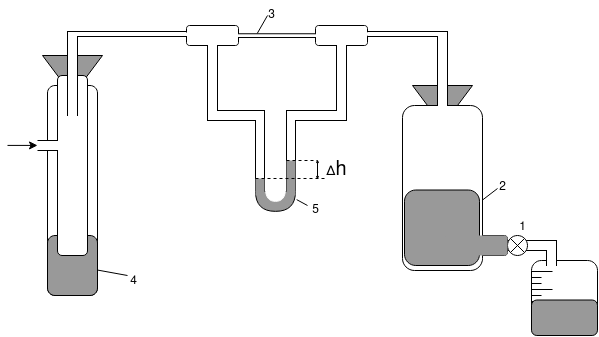
\includegraphics[width=0.5\textwidth]{images/set-up-mean-free-path.drawio.png}
    \caption{\label{fig:setup}Схема на опитна постановка; 1 - кран, 2 - стъклен съд, 3 - капилярка, 4 - изсушител, 5 - диференциален манометър}
    \label{fig:setup}
\end{figure}

\subsection{Задача: Измерване коефициента на вътрешно триене и дължината на свободния пробег на молекулите на въздуха}
Коефициентът на вътрешно триене $\eta$ намираме посредством формула \ref{eq:work-formula} и опитната постановка, илюстрирана на фиг. \ref{fig:setup}. От стъкления съд 2 се пуска да тече вода с постоянна скорост. Това предизвиква различно налягане в тръбичките, като от едната страна на манометъра налягането е атмосферно, а от другата - промененото в следствие на теча на вода, което води до навлизане на повече въздух към съответната страна на диференциалния манометър през капилярката ("отдясно" на илюстрация \ref{fig:setup}). Измерва се обемът на изтеклото количество вода в съда, на който има поставена скала, засича се времето и се изчисляват съответните коефициенти, като резултатите записваме в таблица \ref{tbl:results}. В същата таблица записваме и изчислената средна дължина на свободниня пробег, използвайки формула \ref{eq:lambda}, като от ур.\ref{eq:maxwell} получаваме $\bar{u} = 399.02 \pm 0.07 m/s^2$. В таблица \ref{tbl:constants} са записани константите, използвани при пресмятанията. 

\begin{table}[h]
\begin{center}
\begin{tabular}{|l|l|l|l|l|} \hline
    N & $h_i$, [m] & $t_i$, [s] & $\eta_{i} \cdot 10^{-9}$, [-] & $\bar{\lambda} \cdot 10^{-7}$, [m]\\ \hline
    1 & 0.105 & 39 & 65 \pm 13 & 2.95 \pm 0.02 \\ \hline
    2 & 0.107 & 35 & 59 \pm 12 & 2.70 \pm 0.02 \\ \hline
    3 & 0.067 & 30 & 32 \pm 7 & 1.45 \pm 0.02\\ \hline
    4 & 0.126 & 33 & 66 \pm 14 & 3.00 \pm 0.02 \\ \hline
    5 & 0.094 & 40 & 60 \pm 12 & 2.71 \pm 0.02\\ \hline
\end{tabular}
\caption{\label{tbl:results}Измервания и резултати}
\end{center}
\end{table}


\begin{table}[h]
\begin{center}
\begin{tabular}{|l|l|l|} \hline
    Величина & Стойност и грешка & Мерна единица \\ \hline 
    Обем на изтеклото & (300 \pm 50) \cdot 10^{-6} & m^3 \\ 
    количество вода V & & \\ \hline
    Плътност на въздуха \rho_{air} & (1.293 \pm 0.0005) & kg \cdot m^3 \\ \hline
    Земно ускорение g & (9.81 \pm 0.005) & m/s^2 \\ \hline
    Дължина на капилярка l & (0.134 \pm 0.0005) & m \\ \hline
    Стайна температура T & (293.15 \pm 0.005) & K \\ \hline
    Моларна маса на въздуха \mu_{air} & (0.289 \pm 0.0005) & kg/mol \\ \hline
    Универсална газова константа R & (6.1314 \pm 0.00005) & J \cdot mol^{-1} \cdot K^{-1}\\ \hline
\end{tabular}
\caption{\label{tbl:constants}Константи, използвани при пресмятанията}
\end{center}
\end{table}

Забелязваме, че намерените стойности, макар и всички отразяващи свойствата на едно и също вещество при едни и същи условия не съвпадат в рамките на грешките си. Правим проверка за ламинарно движение, тъй като когато скоростта на движещия се въздух започне да расте, се достига стойност, при която ламинарното движение преминава в турбулентно и формулата на Поазьой вече не е в сила. Тогава потокът $Q$ за турбулентно движещ се флуид и по-малкък от изчисления чрез формула \ref{eq:stream}, тъй като при турбулетно движение $\eta$ е значително по-голям. Видът движение може да се определи посредством числото на Рейнолдс ($Re$), като условието за ламинарно движение на флуид с плътност $\rho$ и коефициент на вътрешно триене $\eta$, който протича в цилиндрична тръба с радиус r е $Re = \frac{r \bar{v} \rho}{\eta} < 1200$, където $\bar{v} = \frac{V}{\pi r^2 t}$ - средната скорост на изтичане. При изчисляването на числото на Рейнолдс за горните резултати се получава число от порядъка $(10-100)\cdot 10^3$, което води до извода, че при направените измервания движението не е било ламинарно и измерванията трябва да се повторят.

\end{document}
